\documentclass{article}
\usepackage[utf8]{inputenc}
\usepackage{graphicx}

% change reference style to [1], remove stupid sorting, language changed so date in ddmmyyyy
\usepackage[backend=biber, style=numeric, sorting=none, language=australian]{biblatex}
\addbibresource{References.bib}

\title{Report}
\author{David Saunders (910995)}
\date{April 2020}

\begin{document}
\maketitle

\begin{abstract} 
    Write abstract here. 4 page report!
\end{abstract}

\tableofcontents

\section{Introduction}

Contextualise the machine-learning problem and introduce the
task and the hypothesis. Make sure to include a few references to previous
work. You should demonstrate an awareness of the research-area.

Write section 1 here \cite{torsney2011tuner} and talk about figure \ref{fig:test}.

\begin{figure}[ht]
    \centering
    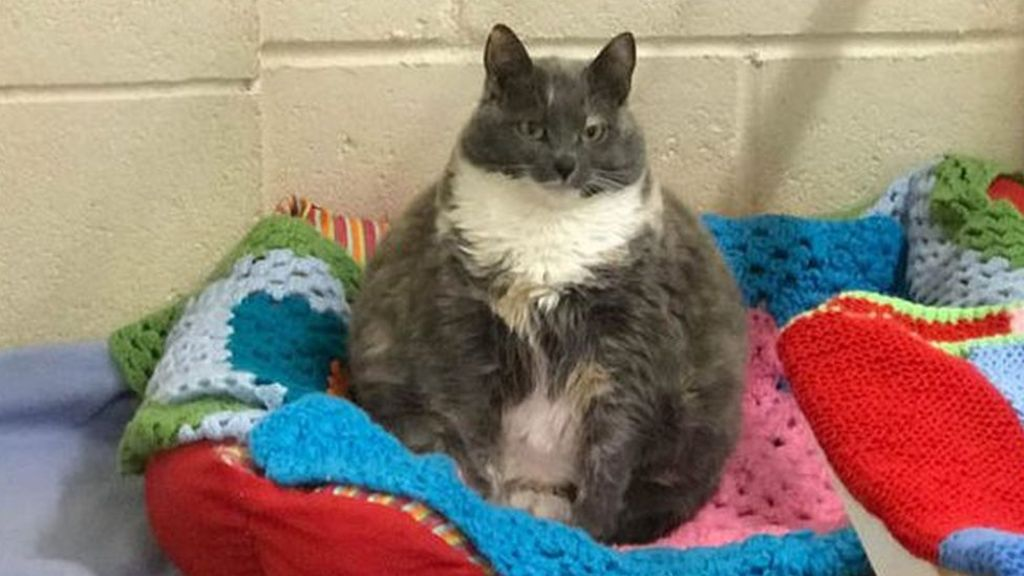
\includegraphics[scale=0.35]{Test.JPG}
    \caption{This will be a figure showcasing some of my work}
    \label{fig:test}
\end{figure}

\section{Methodology}
The model(s) you trained to undertake the task. Any decisions
on hyperparameters must be stated here, including motivation for your
choices where applicable. If the basis of your decision is experimentation
with a number of parameters, then state this.

\section{Results}
Describe, compare and contrast the results you obtained on your
model(s). Any relationships in the data should be outlined and pointed
out here. Only the most important conclusions should be mentioned in
the text. By using tables and confusion-matrices to support the section,
you can avoid describing the results fully.

\section{Discussion and Conclusion}
Restate the task and hypothesis/-ses concisely.
Reiterate the methods used. Describe the outcome of the experiment
and the conclusion that you can draw from these results in respect of the
hypothesis/-ses.

\printbibliography

\end{document}